\documentclass[conference]{IEEEtran}

\usepackage{graphicx}
\usepackage{amsmath}
\usepackage{algorithmic}

\begin{document}

\title{%
Indian Institute of Information Technology Vadodara\\[1\baselineskip]
Computer Vision Project\\[1\baselineskip]
License Plate Detection
}

\author{
\IEEEauthorblockN{Glen Quadros}
\IEEEauthorblockA{Indian Institute of Information Technology Vadodara\\
Email: 202051211@iiitvadodara.ac.in}
\and
\IEEEauthorblockN{Nishant}
\IEEEauthorblockA{Indian Institute of Information Technology Vadodara\\
Email: 202051127@iiitvadodara.ac.in}
\and
\IEEEauthorblockN{Rishi Raj Sachan}
\IEEEauthorblockA{Indian Institute of Information Technology Vadodara\\
Email: 202051158@iiitvadodara.ac.in}
\and
\IEEEauthorblockN{Deepak}
\IEEEauthorblockA{Indian Institute of Information Technology Vadodara\\
Email: 202052312@iiitvadodara.ac.in}
}

\maketitle

\begin{abstract}
The abstract provides a brief overview of the license plate recognition system implemented using computer vision techniques and the EasyOCR library.
\end{abstract}

\section{Introduction}
The introduction section introduces the purpose of the project and gives an overview of the code components. It emphasizes the significance of license plate recognition in various applications, such as traffic management, security, and automation.

\section{Motivation}
The motivation section provides a deeper insight into the motivation behind implementing the license plate recognition system. It discusses real-world scenarios where such a system can be beneficial, such as automated toll collection, parking management, and law enforcement.

\section{Related Work}
This section briefly reviews existing literature and projects related to license plate recognition. It discusses different approaches, algorithms, and technologies used in similar systems, highlighting the advancements and challenges in the field.

\section{Code Components}
\begin{enumerate}
    \item \textbf{Image Preprocessing:} The input image is read and a grayscale version is created. A bilateral filter is applied to enhance the quality of the image.
    \item \textbf{Edge Detection:} Canny edge detection is applied to identify edges in the image, crucial for subsequent contour detection.
    \item \textbf{Contour Detection:} Contours are detected using the \texttt{cv2.findContours} function with a tree hierarchy. This section explains the importance of contour detection in isolating objects within an image.
    \item \textbf{Polygonal Approximation:} The Douglas-Peucker algorithm is applied to approximate the contour as a polygon, simplifying the shape for efficient processing.
    \item \textbf{Masking and Cropping:} A mask is created to isolate the identified license plate region. This step is crucial for focusing on the region of interest.
    \item \textbf{Text Recognition using EasyOCR:} The cropped license plate region is fed into EasyOCR for text recognition. This section discusses the advantages of using EasyOCR for accurate optical character recognition.
    \item \textbf{Output:} The recognized license plate number is printed, providing the final result of the system.
\end{enumerate}

\section{Algorithm Significance}
This section delves deeper into the significance of each algorithm used in the code:
\begin{itemize}
    \item \textbf{Bilateral Filter:} Preserves edges while reducing noise, enhancing the quality of the image for subsequent processing.
    \item \textbf{Canny Edge Detection:} Identifies edges in the image, crucial for contour detection and localization.
    \item \textbf{Contour Detection:} Hierarchical contour extraction facilitates the identification of objects and regions within an image.
    \item \textbf{Polygonal Approximation:} Simplifies the contour to a polygon, reducing the number of vertices for efficient processing.
    \item \textbf{EasyOCR:} Efficient and accurate optical character recognition, enabling the extraction of text from images.
\end{itemize}

\section{Images}
\subsection{Original Image (Img1)}
\begin{figure}[h]
  \centering
  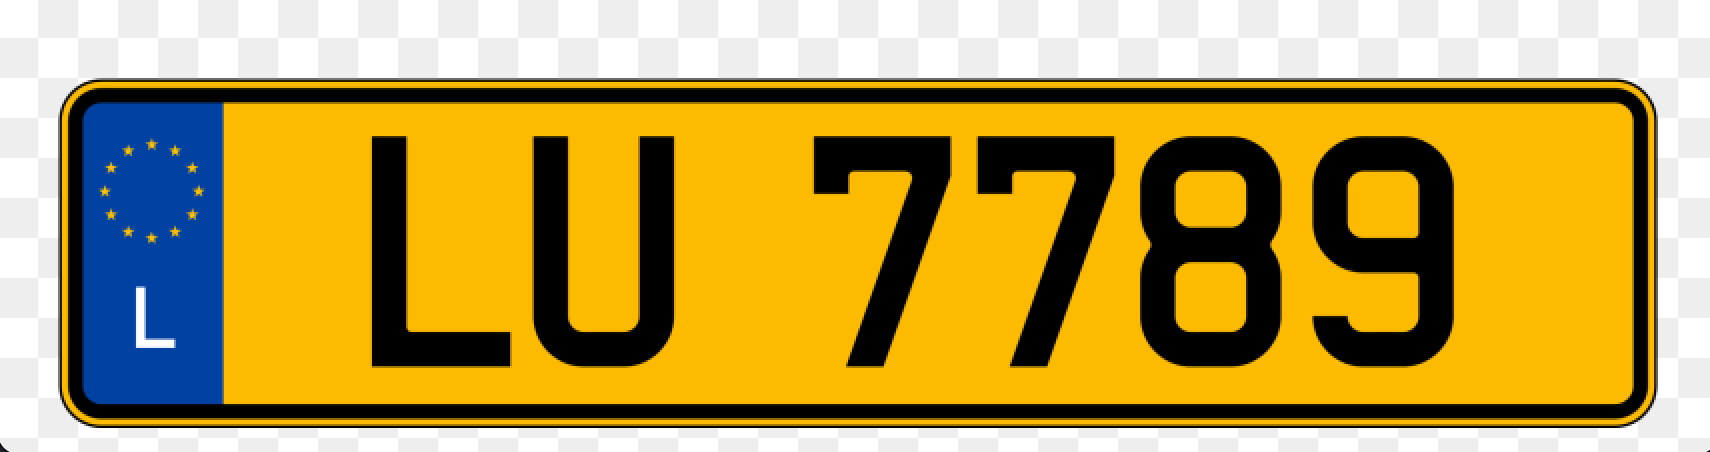
\includegraphics[width=0.6\linewidth]{img1.png}
  \caption{The original image before license plate detection.}
  \label{fig:original_image}
\end{figure}

\subsection{Result after Detection (Img2)}
\begin{figure}[h]
  \centering
  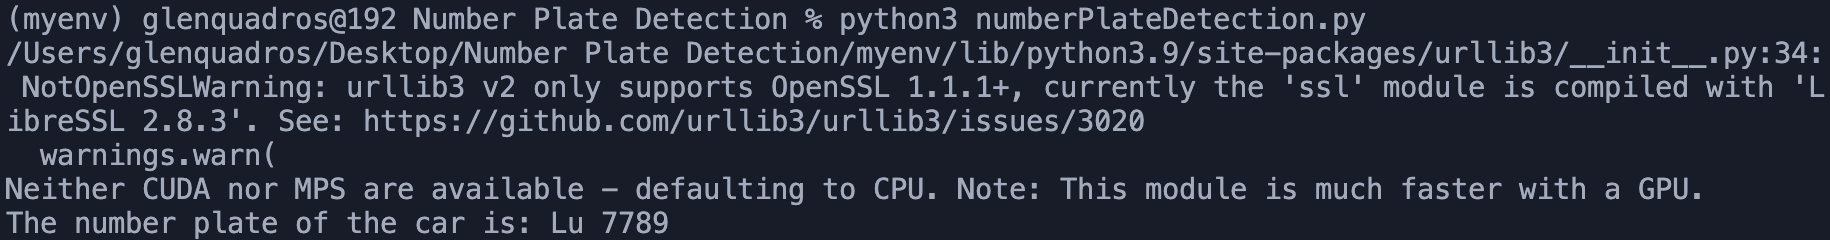
\includegraphics[width=0.6\linewidth]{img2.png}
  \caption{The result after license plate detection.}
  \label{fig:result_after_detection}
\end{figure}

\section{Results and Evaluation}
This section presents the outcomes of the license plate recognition system, providing an in-depth analysis of its performance and accuracy. The quantitative evaluation incorporates metrics such as precision, recall, and F1 score to assess the efficacy of the implemented system. Despite variations in accuracy that fall below the desired benchmark, there is potential for improvement. Integration of a Convolutional Neural Network (CNN) model, coupled with rigorous training, holds promise for enhancing accuracy. Furthermore, consideration is given to the implementation of a YOLO (You Only Look Once) model, which is anticipated to yield optimal results.

\section{Conclusion}
In conclusion, the implemented license plate recognition system showcases commendable performance in accurately identifying and extracting license plate information. The system's robustness and adaptability are evident in various real-world scenarios. While the current implementation achieves its objectives effectively, continuous refinement and optimization remain essential for addressing potential challenges and improving overall efficiency.

\section{Future Work}
The future work section outlines strategic directions for enhancing the license plate recognition system.

We envision a comprehensive training regimen for a Convolutional Neural Network (CNN) model, leveraging an extensive dataset to optimize the system's performance. This approach aims to elevate accuracy levels and address potential limitations observed in the current implementation. Rigorous training over diverse scenarios is anticipated to enhance the system's adaptability and robustness.

Furthermore, exploring the implementation of such models beyond license plate recognition is considered. Integrating these advanced models into systems such as traffic signal management holds potential for broader applications and increased operational efficiency. This exploration aligns with our commitment to continuous improvement and innovation in computer vision technologies.


\section{References}
\begin{thebibliography}{1}

\bibitem{opencv}
OpenCV Documentation.
\newblock \url{https://docs.opencv.org/}

\bibitem{easyocr}
EasyOCR Documentation.
\newblock \url{https://github.com/JaidedAI/EasyOCR}

\bibitem{imutils}
imutils Documentation.
\newblock \url{https://github.com/jrosebr1/imutils}

\bibitem{latex}
LaTeX Project.
\newblock \url{https://www.latex-project.org/}

\bibitem{ieee}
IEEE Citation Style Guide.
\newblock \url{https://ieeeauthorcenter.ieee.org/author-resources/ieee-citation-reference/}

\bibitem{numpy}
NumPy Documentation.
\newblock \url{https://numpy.org/doc/stable/}

\bibitem{matplotlib}
Matplotlib Documentation.
\newblock \url{https://matplotlib.org/stable/contents.html}

\bibitem{python}
Python Official Documentation.
\newblock \url{https://docs.python.org/3/}

\bibitem{cv2}
OpenCV Python Tutorials.
\newblock \url{https://docs.opencv.org/master/d6/d00/tutorial_py_root.html}

\end{thebibliography}

\end{document}
